\chapter{Background \& Objectives}

\section{Introduction}
This project is an investigation into training Artificial Neural Networks for the purpose of image classification and labelling. We will explore alternative approaches in computer vision to solve this problem arriving to the what is considered the current state of the art in machine learning, comparing it to a number of different alternatives, both contemporary but also historical.

\subsection{Motivation}
Perhaps the first question we might wish to ask ourselves is "why we wish to embark on this project in the first place". Computer vision is a field of computer science in essence, involving extracting information and building models of the real world; this might involve sensors, cameras or perhaps even audio.

There are numerous applications and types of computer vision. The problem we are looking in particular is identifying images and labelling them, extracting metadata from the image itself. Naturally this has many applications. Self-driving cars, search engines, and any problem where we need a computer to be able to identify images.

Our interest is particularly related to image acquisition and labelling. Suppose a user has a large set of images and you are looking for a particular one. They know what it is but not its title. Or perhaps its title does not hold semantic meaning to them, but wish to search the semantics of the image itself.

\subsection{Machine Learning and Pattern Recognition}
To solve this problem, computer scientists set out to devise a set of 'rules' and algorithms that were good at solving these problems. Eventually, it became apparent that no single algorithm could solve the problem for all sets of cases as the 'rules' change between cases. The rules that define a cat are different the ones that define a dog and so on, so one would have to write rules for each edgecase. Where you needed to solve this kind of problem one would analyse the data they expect to receive and think of features they are interested in extracting. This approach is still used for some CV problems.

A solution that emerged for this was machine learning $\left(ML\right)$, that is sets of algorithms that could be used to derive the rules based on data. Most machine learning algorithms work by identifying patterns in the data, either via statistical analysis as in Bayesian Learning, or other means. Suppose you have a set of data describing cats and dogs. Cats are small, but there is both small and large types of dogs. Most cats have pointed ears while some dogs have floppy ones. A machine learning algorithm would process a set of examples of cats and dogs, then it would derive patterns that can be used to classify them.

\section{Background}
\subsection{SVMs and other Machine Learning Alternatives}
To use an SVM and most other ML methodologies, you begin by extracting the features you wish to learn from. If for example you are looking at a shape classifier, you would begin by considering what defines your classes. For this example, perhaps the number of edges might be a feature, perhaps the relative length of each straight edge, or maybe the number of detected straight edges.

These can be extracted from an image using computer vision techniques, or in principle, machine learning would be used in a table of features that have already been extracted. Extracting features can be quite challenging on its own and can take a lot of effort. Having extracted the features however,  it is easy to gain insight on the decisions a ML algorithm makes.

\subsection {Artificial Neural Networks}
Artificial Neural Networks$\left(ANN\right)$ are a type of machine learning inspired by the way some biological organisms process stimulus and learn. In essence an ANN is a very naive emulation of a "meat computer", with the biological processes being replaced with mathematical approximations of the actual process of biological neurons.

Being that these are only approximations, they have several components which help them function and emulate select processes of real neurons.

\subsubsection{Advantages and Disadvantages of ANNs}
ANNs have many advantages and disadvantages to conventional ML methods. 

Some of the most important ones include: 
\begin{itemize}
	\item They do not require a feature extraction step
	\item They can easily be applied in many different problems
\end{itemize}
It is possible to apply ANNs in to solve many problems, by just feeding in appropriate training data and get reasonably accurate results in some cases, matching the state of the art for that problem.

As for disadvantages:
\begin{itemize}
	\item They are difficult to train both in terms of requirements and speed
	\item It is comparatively difficult to gain insight on why a neural network has learned something
\end{itemize}
Recent advances in ANNs have greatly improved on both of these areas. GPU compute in particular, has made training quite large neural networks practical, on consumer computers. There is also very active research at the moment in improving insight and visualising neural network decisions. We aim to talk in more detail about all of these later in our report.

\subsubsection{Datasets}
With most methodologies having data to test against is important. With ML, data is what drives the whole process so to produce any sort of solution to this problem one needs to decide on the dataset to use. For classification problems a dataset might be a set of inputs and outputs, separated in a set to train on and a set to test performance against afterwards.

For our network we are looking at datasets with actual images with associated labels. There is several of that type of image dataset, we will discuss them in more detail in a later section of this report.

\section{Analysis}
To complete this project, we must solve a number of problems and answer a number of questions. As part of our analysis we identified some of them, while several others would emerge as we embarked on our project.

\subsection{Types of ML and ANN architectures in use}
To start we should look at what models have been successful in the past for this kind of problem. After all this area has several decades of research behind it which we would not be able to replicate from scratch.

Looking at older results also enables us to get a baseline for what our model might be capable of doing and provides goals to hit or exceed. For this report we will be looking at SVMs, Multi Layer Perceptrons $\left(MLP\right)$ and Convolutional Neural Networks $\left(CNN\right)$

\subsection{Variables to test and optimise}
We need to decide on the architecture of our neural network. For CNN choices appear to be relatively simple, with most networks opting for very similar architectures. However, there are still aspects that can be varied.

We will need to investigate different ways we can vary our model and attributes that we can change in order to limit the scope of the research area. This process involves, reading documentation for our solutions as well as research into the technology we are using to determine the highest value optimisations to make.

\subsection{Are CNNs ready for market?}
One other interesting question to answer, as a conclusion, is whether CNNs are ready to be deployed in commercial products and services. Is it possible to produce something robust enough for such uses?

\section{Research Method}
To tackle any large undertaking, whether it is by a team of a single developer and their tenacity, or involving a team of expert code acrobats working in unison, we as developers, require a set of routines and rituals; this project is no different.

Prompted by a discussion on our Agile Methodologies module, we begun thinking Agile as a solution to this problem. We concluded that Agile would be appropriate to the spirit of our project, however due to this being a solo endeavour, we opted not to adopt any mainstream Agile methodologies. What we did instead is: we took elements we liked from Extreme Programming and combined them with parts of Scrum to create a methodology more closely tailored to our project.

What we needed was a way to drive quick prototyping and creative experimentation in a controlled manner, such that we could plan experiments while maintaining a rudimentary level of quality; while the nature of this project does not necessarily require the end product to be production-ready, since there is no customer nor a production environment. However, poor software quality would only hinder the experimental progress.

In our 'creative experimentation' process, we incorporate the concept of a sprint, but since we expect to go through a small iteration daily, we restrict time to the equivalent of a weekly sprint. Because we lack customers and a product owner, we replace them with our supervisor reporting progress after each week's sprint. The discussion is used to drive the direction and goals of the next sprint.

\begin{wrapfigure}{r}{0.21\textwidth}
	\begin{center}
		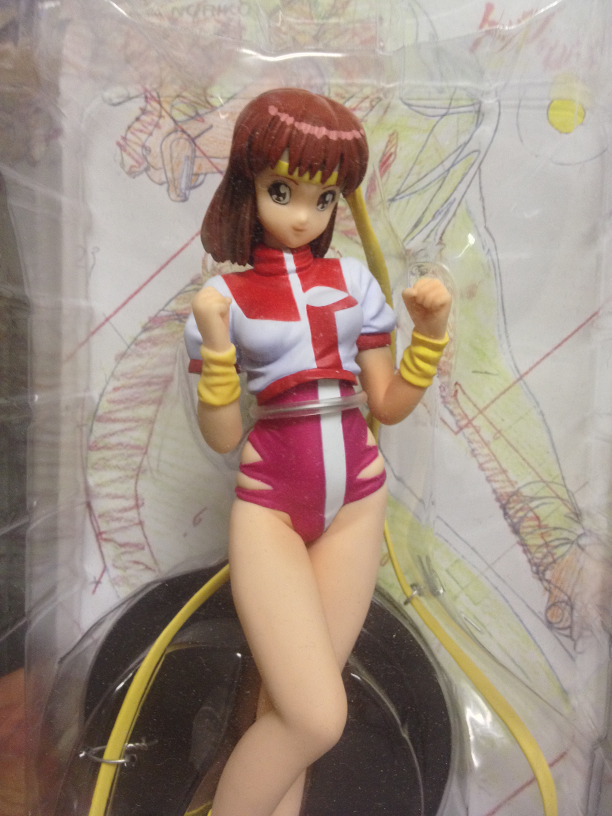
\includegraphics[width=0.19\textwidth]{hard_work_and_guts_programming}
	\end{center}
	\caption{A Pretty Soldier of Hard Work and Guts: Takaya Noriko.}
	\label{hwng}
\end{wrapfigure}

We are also using a form of continuous integration to deploy our changes, and GIT source control to track changes and experiments. We evaluate progress based on feedback from results and from milestones at the end of each 'sprint'. We considered Github issues as well but the were considered superfluous. Polyvinyl Carbonate Figure Debugging was implemented however. See fig. \ref{hwng}

The overall lifecycle looks like this:
\begin{itemize}
	\item First few cycles are exclusively dedicated to research and coming up with a set of requirements for the test infrastructure and programs that need to be developed to drive the project.
	\item After this we focus on designing and testing models with the aid of the basic software we designed in stage 1.
	\item New features will be added as needed to advance the project. Data loading, performance monitoring visualisation etc.
\end{itemize}


For experiments we begin to identify the variables and results we wish to test e.g. size of convolutional filters, then we identify the pre-requisites to run the tests. i.e. do we have the framework to run the experiment, and of course the desired data and whether we can extract them. For the third one we found that there was no need to add more output to run some experiments in our scope. Based on the results of an experiment we decide on what other experiments to run afterwards. Since experiments can take many hours to run, we need to plan a maximum of 2 experiments, a day with a expectation of perhaps doing less on some days or more on others.

Finally, we planned some basic overall schedule we use in 3 major milestones, research, implementation and writeup. Adjustments were to be made based on progress, initial planning was to use 2 weeks for research, 6 weeks for experiments and additional research as needed and 4 weeks for the report.

We have decided to name this methodology 'Hard Work and Guts Programming'. In the spirit of this, we are using this figurine of Takaya Noriko from the 1988 OVA 'Aim for the Top! Gunbuster' as poster child and rubber duck debugging surrogate $\left( fig. \ref{hwng} \right)$